%-----------Thesis Sample for nik-------------------------------------------------
%	Author		:Nikhil M. Dhandre
%	Code date	:12/08/2015
%	Last modi	:13/02/17
%	platform	: STES
%---------------------------------------------------------------------------------

%---------------------------------------------------------------------------------------------------------------------
%--------------------------------------DOCUMENT DECLARATIONS-----------------------------------------------------------
\documentclass[a4paper,12pt]{report}
%---------------------------------------------------------------------------------------------------------------------

%---------------------------------------------------------------------------------------------------------------------
%----------------------------------------PACKAGES USED---------------------------------------------
\usepackage[utf8]{inputenc}

\usepackage{graphicx}
% always load hyperref after amsmath
% \usepackage{amsmath}
% \usepackage{tabularx}
\usepackage[pdftex,
        colorlinks=true,
        urlcolor=blue,       % \href{...}{...} external (URL)
        filecolor=black,     % \href{...} local file
        linkcolor=blue,       % \ref{...} and \pageref{...}
	citecolor=black,
        pdftitle={STES},
        pdfauthor={Nikhil Dhandre},
        pdfsubject={title},
        pdfkeywords={},
%        pagebackref,
%        pdfpagemode=true,
        bookmarksopen=true]{hyperref}
\usepackage{hyperref}
\makeatletter
\def\hyper@refstepcounter#1{%
  \edef\This@name{#1}%
  \ifx\This@name\name@of@eq
    \@ifundefined{theHequation}{%
      \make@stripped@name{\theequation}%
      \let\theHequation\newname
    }{}%
  \fi
  \HyCnt@ProvideTheHCounter{#1}%
  \hyper@makecurrent{#1}%
  \ifmeasuring@
  \else
  %%  \ifmmode\mathopen\bgroup\fi  %% first version of the patch (line I)
    \Hy@raisedlink{%
      \hyper@anchorstart{\@currentHref}\hyper@anchorend
    }%
  %%  \ifmmode\egroup\fi           %% first version of the patch (line II)
  \fi
  \ifmmode\mathopen{}\fi           %% second version: THIS LINE ADDED IN PATCH
}
\makeatother
\usepackage{anysize}
\usepackage{latexsym}
\usepackage{pictex}
\usepackage{fancyvrb}
\usepackage{fancyhdr}
\usepackage{color}
\usepackage{multirow}% http://ctan.org/pkg/multirow
\usepackage{hhline}% http://ctan.org/pkg/hhline
% lscape.sty Produce landscape pages in a (mainly) portrait document.
\usepackage{lscape}
\usepackage{gensymb}
\usepackage{textcomp}
%\usepackage{subfigure}
\usepackage{rawfonts}
\usepackage{geometry}

% Page border
%---------------------------------------------------------------------------------------------------------------------


%---------------------------------------------------------------------------------------------------------------------
%----------------------------------MARGIN DECLARATIONS--------------------------------------------------------------

\marginsize{37mm}{25.4mm}{25.4mm}{32mm}
\linespread{1.3}
\pagestyle{headings}

%---------------------------------------------------------------------------------------------------------------------
%---------------------------------------------------------------------------------------------------------------------

%--------------------- configure file------------------------------------------------
%---------------------------------------------------------------------------------------------------------------------


\def\title{DAM \& WEATHER PARAMETERS\\[.3CM] MONITORING SYSTEM}
\def\TitleHead{Dam \& Weather Parameters Monitoring System}
\def\report{Dissertation Report} % Seminar I, II,/Project stage-I 
\def\REPORT{DISSERTATION REPORT} % SEMINAR I, II,/PROJECT STAGE-I 

\def\dept{Department Of E\&TC Engineering}
\def\DEPT{DEPARTMENT OF E\&TC ENGINEERING}

\def\dg{Master of Engineering (E\&TC)}
\def\DG{MASTER OF ENGINEERING (E\&TC)}

\def\branch{VLSI \& Embedded Systems}
\def\BRANCH{VLSI \& EMBEDDED SYSTEMS}

\def\author{Nikhil Dhandre}
\def\AUTHOR{NIKHIL DHANDRE}
\def\GEN{HIM}

\def\rollno{525003}

\def\email{nik.digitronik@live.com}
\def\GUIDE{PROF. D. E. UPASANI}
\def\guide{Prof. D. E. Upasani}

\def\pgco{Prof. D. E. Upasani}
\def\hod{Prof. D. E. Upasani}
\def\princi{Prof. D. E. Upasani}

\def\college{Sinhgad Institute of Technology \& science}
\def\COLLEGE{SINHGAD INSTITUTE OF TECHNOLOGY \& SCIENCE}

\def\uni{Savitribai Phule University of Pune}
\def\UNI{SAVITRIBAI PHULE UNIVERSITY OF PUNE}

%---------------------------------------------------------------------------------------------------------------------


%---------------------------------------------------------------------------------------------------------------------
%-----------------------------------DOCUMENT START FROM HERE---------------------------------------------

\begin{document}


\pagenumbering{roman}	% ROMAN NUMBERING FOR START UP

%--------------------------------------newcommand ---------------------------------------------------------------------
\newcommand{\HRule}{\rule{\linewidth}{0.5mm}} % New command to make the lines
\renewcommand\bibname{References}

%---------------------------------------------------------------------------------------------------------------------
%--------------------------------TITLE PAGE--------------------------------------
\begin{titlepage}
\newgeometry{left = 2cm,right = 1cm,bottom = 1cm,top = 1cm}
\thispagestyle{empty}
\begin{center}
\textbf{A \\[.2cm] \REPORT \\[.2cm] ON}
\\[.3cm]
\textbf{\LARGE \title }
\\[.3cm]
\textbf{SUBMITTED TO THE \UNI, IN
THE PARTIAL FULFILLMENT OF REQUIREMENTS FOR THE
AWARD OF THE DEGREE \\[.2cm] OF }
\\[.2cm]
\textbf{\Large \DG \\[.2cm] (\BRANCH)}
\\[.3cm]
\emph{By:}
\\[.2cm]
\textbf{\large \AUTHOR}
\\
\textbf{ROLL NO: \rollno}
\\[.5cm]

\emph{UNDER THE GUIDANCE OF:}
\\[.2cm]
\textbf{\large \GUIDE}
% \\[.1cm]
% \textbf{\large Shri P. D. Kamalasekaran}
% \\(Scientist-D)
\\[1.5cm]

\includegraphics[width=4cm]{figures/scoe_logo.png}
\\[1.5cm]

\textbf{\Large \DEPT} 
\\[.3cm]
\textbf{SINHGAD TECHNICAL EDUCATION SOCIETY’S}
\\[.2cm]
\textbf{\Large \COLLEGE}
\\[.3cm]
\textbf{NARHE (AMBEGAON), OFF WESTERLY BY PASS PUNE MUMBAI
\\ EXPRESSWAY, NARHE, PUNE - 411 041} \\[1cm]
\textbf{\Large YEAR 2016-17} 
\end{center}
\clearpage
\restoregeometry
\end{titlepage}

%---------------------------------------------------------------------------------------------------------------------
%---------------------------------------------------------------------------------------------------------------------
%---------------------------------------------------------------------------------------------------------------------
%---------------------------------------------------------------------------------------------------------------------



%---------------------------------------------------------------------------------------------------------------------
%-----------------------------CERTIFICATE PAGE--------------------------------------
\newpage
\newgeometry{left=32mm,right=25.4mm,bottom=32mm,top=25.4mm}
\thispagestyle{empty}
\vspace{1cm}
\section*{\begin{center} {\huge{CERTIFICATE}}\end{center}}
\vspace{.5cm}
\begin{center}

\textsc{This is to certify that the \report \ entitled }\\[.3cm]
{\Large \bf "\title"}\\[.3cm]
\emph{Submitted By} \\[.2cm]
{\bf \large \author (\rollno)}
\end{center}

\textsc{Is a Bonafide work carried out by \GEN \,under the
guidance of \GUIDE and it is approved for the partial fulfillment of the
requirement of the SAVITRIBAI PHULE PUNE UNIVERSITY for the award of} 

\begin{center}
{\textbf{The \DG \\ (\BRANCH)}} 
\end{center}

\textsc{This \report \, has not been earlier submitted to other Institute or University for the award of
any degree or diploma.}
\vspace{1.5cm}


\begin{center}

\footnotesize
$$
\begin{array}{c c c}
\hspace{5cm} \hfil	& \hspace{5cm} \hfil	&\hspace{5cm} \hfil\\
\bf(\guide) 	&  \bf \pgco	&\bf \hod \\
Guide 		& PG Coordinator& HOD	\\
E\&TC		& E\&TC		&E\&TC \\
\\
\\
\\
\\
\textbf{(External Examiner)} & &\textbf{Principal}\\
\end{array}
$$
\end{center}

% \begin{tabular}{c c c c c c c}
% \hspace{1cm}		& &\hspace{1cm}		&\hspace{.1cm}	&\hspace{1cm}		&	&\hspace{1cm}	\\
% \bf\guide 		&  		&\bf Kamal Shekaran	&		&\bf \pgco		& 		&\bf \hod 	\\
% Guide 			& 		& External Guide	&		&PG Coordinator		& 		& Head		\\
% Department of  		& 		& Scientist-D, 		&		&CN, E\&Tc 		& 		& Department of  \\
% E\&TC			&		&CWPRS, Pune		&		&			&		&E\&TC		\\
% 			& 		&			&		&			&		&		\\
% 			&		&			&		&			&		&		\\
% 			&		&			&		&			&		&		\\
% 	& 	&			&		&			&		&\textbf{Principal}\\
% 			& 		&			&		&			&		&S.C.O.E. Pune 
% \end{tabular}


\vspace{1cm}
\begin{flushleft}
 Place: Pune \\
 Date\,: \today
\end{flushleft}
\clearpage
\restoregeometry

%---------------------------------------------------------------------------------------------------------------------
%---------------------------------------------------------------------------------------------------------------------




%---------------------------------------------------------------------------------------------------------------------
%---------------------------------DEDICATION  PAGE-----------------------------------------
%\newpage
%\chapter*{}
%\thispagestyle{empty}
%\vspace*{2.5in}
%\begin{center}
%Dedicated to\\
%my mother\\ 
%{\bf adsfsafadsf}\\
%\vspace{0.25in}
%and\\
%my father\\
%{\bf dsfsadfasf}
%\end{center}
%---------------------------------------------------------------------------------------------------------------------
%---------------------------------------------------------------------------------------------------------------------


%---------------------------------------------------------------------------------------------------------------------
%------------------ACKNOWLEDGMENT PAGE-------------------------------------------------------------------------------

\newpage
\vspace{1.5cm}
\section*{\begin{center}\Huge{Acknowledgment}\end{center}}
\addcontentsline{toc}{chapter}{\quad\,\,{Acknowledgment}}
%\thispagestyle{empty}
\hfill 

Any accomplishment requires the effort of many people and this work is no different. I find great pleasure in expressing my deep
sense of gratitude towards all those who have made it possible for me to present dissertation work.

I would like to express a sincerest gratitude to my guide \textbf{\guide} for his dynamic and valuable guidance. I am grateful to him for constant
encouragement in the fulfillment of the dissertation. This work is a result of combined effort put in by my guide for providing me with 
all necessary infrastructure and facilities to complete work.

I would like to thanks my PG Co-ordinator \textbf{\pgco} for his time to time guidance and best suggestion. I am also very thankful to Head 
of Department of Electronics \& Telecommunication \textbf{\hod} for his valuable guidance time to time. I am highly thankful to Principle
\textbf{\princi} for his valued support and faith on me.


I am also thankful to all Staff Members who extended the preparatory steps of this dissertation work. I would also  like to express
appreciation and thanks to all my friend who unknowingly assisted me with their valuable suggestions and support. I wood also like
to thank those who have directly or indirectly guided me.\\[2cm]

\begin{flushright}
\bf \author
\end{flushright}
%---------------------------------------------------------------------------------------------------------------------
%---------------------------------------------------------------------------------------------------------------------


%---------------------------------------------------------------------------------------------------------------------
%-----------------TABLE OF CONTENTS AND LIST PAGEES------------------------------------------------------------
\listoffigures
\addcontentsline{toc}{chapter}{\quad\,\,{List of Figures}}
\listoftables
\addcontentsline{toc}{chapter}{\quad\,\,{List of Tables}}
\tableofcontents
%-----------------------------------------------------------------------
%---------------------------------------------------------------------------------------------------------------------

%---------------------------------------------------------------------------------------------------------------------
%------------------------ -  NOMENCLATURE AND ABBRIVATION  -------------------------------------------------
\newpage
\vspace{1.5cm}
\section*{\begin{center} {\Huge{Nomenclature and Abbreviation }}\end{center}}
\thispagestyle{empty}
\addcontentsline{toc}{chapter}{\quad\,\,{Nomenclature and Abbreviation }}

\begin{table}[h]
  \begin{tabular}{l l c}
 \bf ADC & Analog to Digital Converter&\\
 \bf AH & Absolute Humidity &$(grams/m^3)$\\
 \bf CSV & Comma Separated Values\\
 \bf DWPMS & Dam \& Weather Parameters Monitoring System\\
 \bf GDP & Gross Domestic Product\\ 
 \bf GUI & Graphical User Interface\\
 \bf IoT & Internet of Things&\\
 \bf M2M & Machine to Machine Communication&\\
 \bf RFID & Radio Frequency Identification &\\
 \bf RH & Relative Humidity &$(\%)$\\
 \bf RTDS & Real Time Decision Support&\\
 \bf RTDSS & Real Time Decision Support System&\\ 
 \bf RTD & Resistance Temperature Dependant&\\ 
  \bf SCADA & Supervisory Control and Data Acquisition\\
\bf SHIS & Smart Home Information System &\\

 \bf DB & Database &\\
 \end{tabular}
\end{table}

%---------------------------------------------------------------------------------------------------------------------

%---------------------------------------------------------------------------------------------------------------------
%------------------------- ABSTRACT PAGE -------------------------------------------------
\newpage
\vspace{1.5cm}
\section*{\begin{center} {\Huge{Abstract}}\end{center}}
\thispagestyle{empty}
\addcontentsline{toc}{chapter}{\quad\,\,{Abstract}}
Authentic time dam and weather parameters monitoring are today's need. The nowadays dam authority is facing problems 
related to the dam and weather parameter monitoring. Up to now most of the smaller dams are manually monitored and 
sending data with normal ways, this manual observation and transmission results in a time lag, between the data observed 
in dam site and decision taking level. This sometimes causes loss of beneficial real time data. Researchers want observed 
data to be readily available for research purpose as well as monitor the authentic time changes in various parameters. 
Common people, mainly farmers are unaware about these parameters like rainfall, Dam water level and gate status. This project 
will help to reduce these problems faced by Dam authority, researchers as well as common people (farmers). The concept of 
this system is to develop a web portal which will monitor and give authentic time parameters related to Dam and weather conditions. 
It also provides facility of downloading CSV file of recorded parameters readings. GUI Software developed in this system will provide 
two types of facility Autopilot mode and Manual mode. At back end of the software it takes parameter information from the 
related sensors and dumps it into the database. The dumped data can be used for maintaining a database and further decision making. 
This proposed scheme basically works on Internet of Things (IoT), so that data sharing can be possible utilizing web data base.
\\[1cm]
\textbf{Index Terms:} Dam parameters, GUI, Internet of Things (IoT), monitoring system, weather parameters, web-portal.

%---------------------------------------------------------------------------------------------------------------------



%---------------------------------------------------------------------------------------------------------------------
%---------------------------------------------------------------------------------------------------------------------

%-----------------------PAGE STYLE DECLARATIONS---------------------------------------------------------

\newpage
\pagenumbering{arabic} % START NORMAL NUMBERING OF PAGE FROM HERE
\pagestyle{fancy}

\fancyhead[LE]{\leftmark}
\lhead{\TitleHead}
\fancyhead[RO]{\rightmark}
\fancyhead[RE]{}

\rfoot{\thepage}
\cfoot{\footnotesize{SITS , NARHE , PUNE-41 (E\&TC ENGINEERING)}}

\renewcommand{\headrulewidth}{0.1pt}
\renewcommand{\footrulewidth}{0pt}

\renewcommand{\sectionmark}[1]{%
\markright{\it \thesection \ #1}{}}

\renewcommand{\chaptermark}[1]{%
\markboth{\it \chaptername \ \thechapter.\ #1}{}}
%---------------------------------------------------------------------------------------------------------------------











%---------------------------------------------------------------------------------------------------------------------
\chapter{INTRODUCTION}
%---------------------------------------------------------------------------------------------------------------------
\label{CH:introduction}

Water and Weather are playing a vital role in our daily lives, these are important factors that can not be neglected.
The Economy of India is the seventh-largest in the world, the agricultural sector is the largest employer in India's 
economy but contributes to a declining share of its GDP (17\% in 2013-14). 
Hence to cater that dams are built. Dams can fulfill these need, as they are source of water and hydro-electric power. 
\newline

Now a days dam authority facing problems regarding the dam and weather parameters monitoring as most of small dam till using
manual data observation and transmission. Older transmission system make much more difference in decision making.
\newline

Dam researchers want to monitor dam data continuously to observe the changes in parameters. They want centralize database 
so they can perform operation on well collected and organize data. For research purpose in India centralize database not available up to now.
Presently researchers request to dam authority for data. It means that data availability is major problem for them. 
\newline

Normal people like farmers also unaware about these parameters 
like water level, gate opening, amount of rainfall, temperature, humidity; so they are facing many problems.
Due to heavy rainfall, the water level of dam increases suddenly due to which the Dam authority have to open the gates to prevent the dam from the risk of uncertainty issues. Also due to this the people living in nearby villages have to face a serious problem like flood in their farms. 
When back water of dam increases above its threshold level(danger level) it may cause damage to farms, villages, industries located nearby and lastly the lives of the people living nearby.
\newline

Manual data observation and transmission results in a considerable time
lag, between data observed in field and its communication to decision making level
which sometime leaves little time, so there may be a possibility of losing a real time data.
The proposed scheme will help to reduce such problems.
\newline

This system will help to reduce these problems which faced by Dam authority, researchers as well as common people like farmers. 
\newline

The conception about this system is to develop a web portal which will monitor and provide authentic time parameters related to Dam and weather like water level, rain fall, dam gate position, temperature, humidity etc. 
\newline

In observation part the smart controller provides facility of dumping sensor observation values directly into database with specific time interval. It provides the facility of SMS for providing data. Also the system has an alarm which will give alerts and will help in knowing critical conditions.
\newline

As it is basically based on Internet data sharing with the help of web database, like weather parameters for Meteorological department, dam parameters to government authority etc, the Government of India wants to monitor the real time water level of reservoirs. Hence this work will help in Digital India Mission.

\section{Relevance}
This system will make easy monitoring of Dam and Weather parameters. 
Which will help to Dam authority, Dam researchers and normal people. 
Real Time Decision Support (RTDS) will help for various decision making related to parameters.

\section{Objectives}
Following are the objectives of this project:
\begin{itemize}
 \item To monitor \& Analyse Dam Parameters
 \begin{itemize}
  \item Dam authority
  \item Dam researchers
  \item Normal People
 \end{itemize}
 \item To monitor \& Analyse weather Parameters
 \item To develop GUI software
 \item To provide Real Time Decision Support (RTDS)
 \item To data sharing with remote systems
 \item To develop finished Product
 \item To Publish Paper in good Journals 
\end{itemize}
%---------------------------------------------------------------------------------------------------------------------







%---------------------------------------------------------------------------------------------------------------------
\chapter{LITERATURE REVIEW}
%---------------------------------------------------------------------------------------------------------------------
\label{CH:literature_review}

The term “Internet of Things” was first documented by a British visionary, Kevin Ashton, in 1999.
Typically, IoT is expected to offer advanced connectivity of devices, systems, and services that goes beyond 
machine-to-machine communications (M2M) and covers a variety of protocols, domains, and applications.
The interconnection of these embedded devices (including smart objects), is expected to usher in automation in nearly all fields, 
while also enabling advanced applications like a Smart Grid. 
\cite{rfid:iot}
\newline

Kevin Ashton wrote article in RFID journal that He could be wrong, but he fairly sure the phrase 
"Internet of Things" started life as the title of a presentation he made at Procter and Gamble in 1999. Linking the 
new idea of RFID in P and G's supply chain to the then-red-hot topic of the Internet was more than just a good way to get executive attention. 
It summed up an important insight one that 10 years later, after the Internet of Things has become the title of everything from 
an article in Scientific American to the name of a European Union conference, is still often misunderstood.
\cite{rfid:iot}
\newline

H. Li and X. Xing discloses the architecture of an internet of things (IOT). The architecture includes multiple levels of IOT service platforms,
also discloses a method for implementing an IOT service. The method includes the steps of the superordinate IOT service platform providing 
management for one or more of subordinate IOT service platform, special service platform and service gateway, wherein the management includes 
one or more of registration, login, logout, data synchronization. With this the deployed industries or special service 
platforms can be integrated into a unified architecture, thus lightening the burden of the IOT service platforms.
\cite{P-IoT:EP2566281A1}
\newline

D. A. Bagade  proposed plan under "Maha krishna" for real time data acquisition and reservoir operation in Maharashtra. In that proposed Real Time Decision Support 
System (RTDSS) with SCADA network for data connectivity and covers the  Automated rainfall station, Automated full climate station, Automated discharge measurement,
Web portal giving the total current data about discharge, water lavel, rainfall about reservoir.
\cite{RTDSS:BAGADE}
\newline

M. Wang et al. proposed a smart control system base on the technologies of internet of things has been proposed to solve
how to manage and control these increasing various appliances efficiently and conveniently so as to achieve more comfortable, 
security and healthy space at home. To manage all appliances in a smart home, he develop a smart home information system (SHIS) with web technologies.
\cite{IoT:home-automation}
\newline

B. Kang et al. proposes an IoT-based monitoring system using a tri-level context making model for context-aware services in smart homes
as data acquisition and information analysis through various sensors will play a crucial role. The necessary technology is one that collects 
and analyzes much different information around us through various sensors.
\cite{IoT:trilevel}
\newpage
\begin{table}[h!]
\caption{Literature Survey}
\centering
 \begin{tabular}{||l|l|l|} \hline
\bf Contributors 	& \bf Parameter & \bf Significance \\ \hline
Kevin Ashton 		& IoT		&advanced connectivity of devices,\\ 
			&		&systems, and services that goes \\
			&		&beyond M2M communications and covers\\ 
			&		& a variety of protocols, domains, and \\
			&		&applications \\ \hline
H. Li and X. Xing 	& IoT		& Architecture of an internet of things \\ \hline
D. A. Bagade		& RTDSS		& SCADA network for data connectivity\\
			&		& Web Technologies \\ \hline
M. Wang et al.		& Smart Control & smart home information system \\
			&System		&(SHIS) with web technologies \\ \hline
B. Kang et al.		& Tri-level Model& It is technology that collects and\\ 
			&		&analyzes much different information \\
			&		&around us through various sensors.\\ \hline
\end{tabular}
\end{table}



%---------------------------------------------------------------------------------------------------------------------









%---------------------------------------------------------------------------------------------------------------------\
\chapter{COMPONENT SELECTION}
%---------------------------------------------------------------------------------------------------------------------\
\label{CH:comp_selection}


\section{Introduction}
\subsection{Good Sensor}
The two most important characteristic of a sensor are:
\begin{itemize}
 \item \textbf{Precision -} The ideal sensor will always produce the same output for the same input.\cite{Adafruit}  
 \item \textbf{Resolution -} A good sensor will be able to reliably detect small changes in the measured parameter.\cite{Adafruit}
\end{itemize}

\begin{figure}[h!]
\centering
 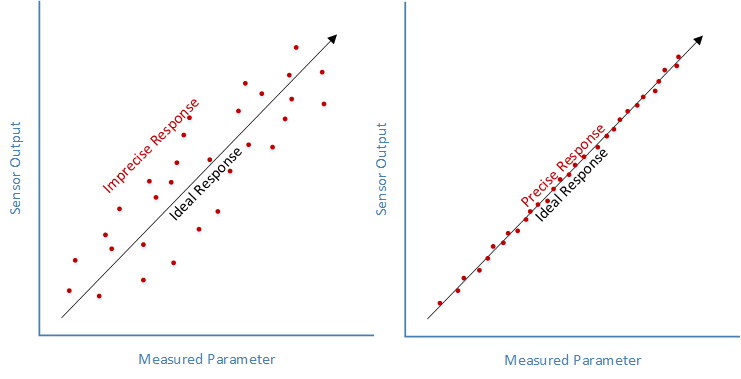
\includegraphics[width=.80\textwidth]{figures/sensors_Precision.png}
 \caption{Sensor Precision }
\end{figure}

\subsection{Affects of Precision}
\begin{itemize}
 \item \textbf{Noise -} All measurement systems are subject to random noise to some degree.  Measurement systems with a low Signal to Noise Ratio will have problems making repeatable measurements.  In the diagrams above, the sensor on the right shows much better precision than the noisy one on the left.\cite{Adafruit}
 \item \textbf{Hysteresis -} Some types of sensors also exhibit hysteresis.  The sensor will tend to read low with an increasing signal and high with a decreasing signal as shown in the graph below.  Hysteresis is a common problem with many pressure sensors.\cite{Adafruit}

 \begin{figure}[h!]
 \centering
  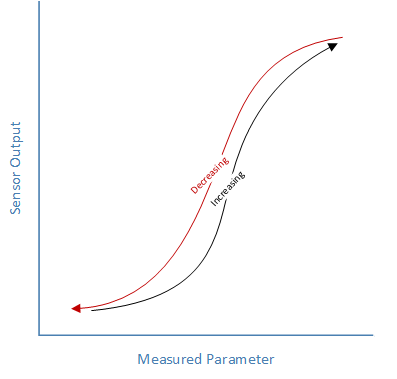
\includegraphics[width=8cm, height=7cm]{figures/sensors_Hysteresis.png}
  \caption{Sensors Hysteresis }
 \end{figure}
\end{itemize}

\subsection{Other Important Qualities In a Sensor}
Precision and resolution are the real 'must have' qualities.  But there are a couple of other 'nice-to-have' qualities:
\begin{itemize}
 \item \textbf{Linearity -} A sensor whose output is directly proportional to the input is said to be linear.  This eliminates the need to do any complex curve-fitting and simplifies the calibration process.
\item \textbf{Speed -} All else being equal, a sensor that can produce precise readings faster is a good thing to have.
\begin{figure}[h!]
 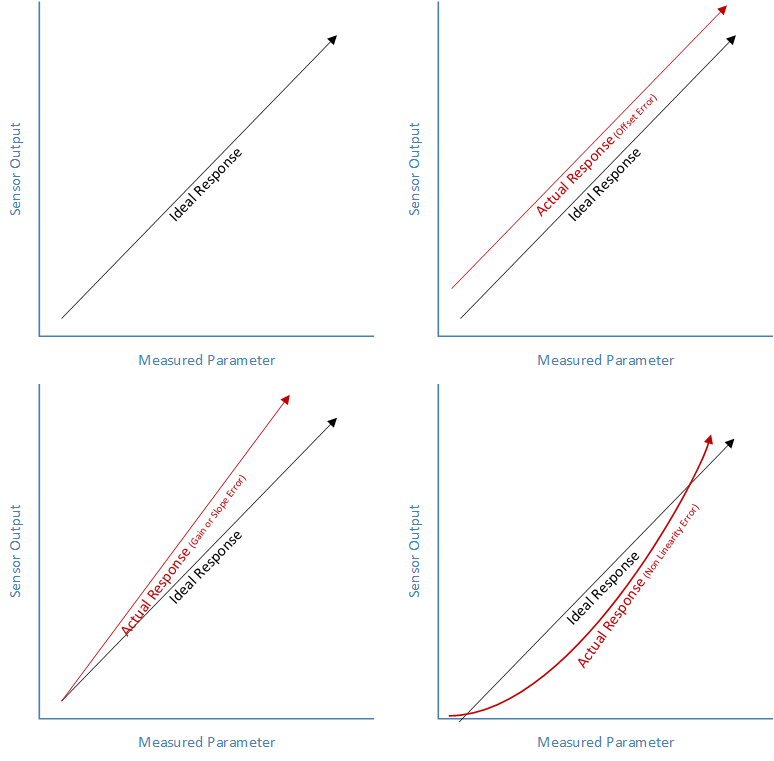
\includegraphics[width=\textwidth]{figures/sensors_Errors.png}
 \caption{Sensors Errors}
\end{figure}
\end{itemize}

\textbf{Accuracy} is a combination of precision, resolution and calibration.  
If you have a sensor that gives you repeatable measurements with good resolution, you can calibrate it for accuracy.\cite{Adafruit}
\newline

\textbf{Digital sensors} are calibrated at the factory to some extend  but, digital sensors are still subject to manufacturing 
and operating condition variability.  For critical measurements, you need to calibrate the total system.\cite{Adafruit}

\pagebreak
%---------------------------------------------------------------------------------------------------------------------\




\section{Raspberry Pi}

 \begin{figure}[h]
 \centering
  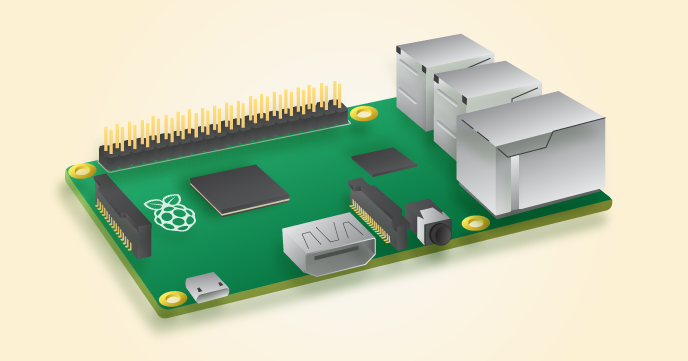
\includegraphics[width=\textwidth]{figures/Pi_2_Model_B.png}
  \caption{Raspberry Pi 2 Model B.}
 \end{figure}

The Raspberry Pi is a low cost, \textbf{credit-card sized computer} that plugs into a computer monitor or TV, and uses 
a standard keyboard and mouse. It is a capable little device that enables people of all ages to explore computing, and 
to learn how to program in languages like Scratch and Python. It’s capable of doing everything you had expect a desktop 
computer to do, from browsing the Internet and playing high-definition video, to making spreadsheets, word-processing, 
and playing games.\cite{instructables_rpi}
\newline

The Raspberry Pi Foundation is a registered educational charity (\textbf{registration number 1129409}) based in the UK. 
Foundation’s goal is to advance the education of adults and children, particularly in the field of computers, 
computer science and related subjects.
\begin{landscape}
\begin{table}[h]
\caption{Available Raspberry Pi Models }
\begin{tabular}{|l|c|c|c|c|c|}\hline
Attribute& Model A	& Model A+	& Model B	& Model B+	& 2 Model B	\\\hline
SoC	& Broadcom	& Broadcom	& Broadcom	& Broadcom	& Broadcom	\\
	& BCM2835	& BCM2835	& BCM2835	& BCM2835	& BCM2835	\\ \hline
CPU	& 700MHz	& 700MHz	& 700MHz	& 700MHz	& 900MHz 	\\
	& ARM1176JZF-S	& ARM1176JZF-S	& ARM1176JZF-S	& ARM1176JZF-S	& Quad-core ARM Cortex-A7 \\ \hline
GPU	& Video Core IV	& Video Core IV	& Video Core IV	& Video Core IV	& Video Core IV	\\ \hline
RAM	& 256 Mb	& 256 Mb	& 512 Mb	& 512 Mb	& 1 Gb		\\ \hline
USB	&1		&1		&2		&4		&4		\\ \hline
Video	& RCA, HDMI	& Jack, HDMI	& RCA, HDMI	& Jack, HDMI	& Jack, HDMI	\\ \hline
Audio 	& Jack, HDMI	& Jack, HDMI	& Jack, HDMI	& Jack, HDMI	& Jack, HDMI	\\	\hline
Boot	& SD		& MicroSD	& SD		& MicroSD	& MicroSD	\\ \hline
\end{tabular}
\end{table}
\end{landscape}

%---------------------------------------------------------------------------------------------------------------------



\section{Temperature Sensors}
There are mainly three type of temperature sensors as fallow:
\begin{enumerate}
  \item Thermocouple
  \item RTD
  \item Thermistor 
\end{enumerate}

\subsection{Thermocouple}
A Thermocouple is a sensor used to measure temperature. Thermocouples consist of two wire legs made from different metals. 
The wires legs are welded together at one end, creating a junction. This junction is where the temperature is measured. 
When the junction experiences a change in temperature, a voltage is created. 
The voltage can then use to calculate the temperature.

\subsection{RTD}
Resistance Temperature Detectors (RTDs) are sensors that measure temperature by correlating the resistance of the RTD element 
with temperature. Most RTD elements consist of a length of fine coiled wire wrapped around a ceramic or glass core.

\subsection{Thermistor}
Thermistors are special solid temperature sensors that behave like temperature-sensitive electrical resistors. 
No surprise then that their name is a contraction of "thermal" and "resistor".

\subsection{Comparison}

\begin{table}[h]
\centering
\caption{Temperature sensors comparison}
 \begin{tabular}{||l|c|c|c|} \hline
\bf Attribute 		& \bf Thermocouple 	&  \bf RTD 		&\bf  Thermistor	\\ \hline
Cost 			& Low		& High		& Low 		\\ \hline
Temperature Range	& Very wide 	& Wide 		& Short to medium\\
			& -350\textdegree F - +3200\textdegree F	&-400\textdegree F - +1200\textdegree F	&-100\textdegree F - +500\textdegree F \\ \hline
Interchange ability	& Good		& Excellent	& Poor to fair \\ \hline
Long-term Stability	& Poor to fair	& Good		& Poor \\ \hline
Accuracy		& Medium	& High		& Medium \\ \hline
Repeatability		& Poor to fair	& Excellent	& Fair to good \\ \hline
Sensitivity (output)	& Low		& Medium	& Very high \\ \hline
Response		& Medium to fast& Medium	& Medium to fast \\ \hline
Linearity		& Fair		& Good		& Poor \\ \hline
Self Heating		& No		& Very low 	& High \\ \hline
Point (end) Sensitive	& Excellent	& Fair		& Good \\ \hline
Lead Effect		& High		& Medium	& Low \\ \hline
Size/Packaging		& Small to large &small to medium & Small to medium \\ \hline
 \end{tabular}

\end{table}

From above comparison of the main type of sensor \textbf{RTD} is best solution for our project as it has a excellent Interchange ability, 
good long term stability, high accuracy and maintaining linearity with medium output sensitivity.

%---------------------------------------------------------------------------------------------------------------------\
\section{Humidity Sensor}
According to the measurement units, humidity sensors are divided into two types: 
\begin{enumerate}
 \item Relative humidity(RH)sensors 
 \item Absolute humidity(moisture) sensors
\end{enumerate}

\subsection{Relative humidity Sensors}
Principle is Ratio of mass(vapour) to mass(saturated vapour) or ratio of actual vapor pressure to saturation vapor pressure.
$$ RH = \frac{Mass (vapour)}{Mass (Saturated vapor)}
$$
It is measure in percentage (\%)

\subsection{Absolute humidity sensors}
Principle is Ratio of mass(vapor) to volume.
$$ AH = \frac{Mass (vapour)}{Volume}
$$
It is measure in $ grams/m^3$
\newpage
\begin{landscape}
 
\begin{table}[h]
\centering
\scriptsize  
\caption{Available Temperature and Humidity Packages Comparison for experimental setup}
 \begin{tabular}{||l|c|c|c|c|c|c|c|c|}\hline
\multirow{2}{*}{\bf Attribute} & \multicolumn{8}{c|}{\bf Sensors} \\
\hhline{~--------}
		&\bf LM35	&\bf HR202L	&\bf DS18B20	&\bf DHT22	&\bf HTS221	&\bf RHT03	&\bf AM2001	&\bf LMT87\\ \hline
Type		& Temp		& Humi		&Temp		&Temp/humi	&Temp/humi	&Temp/humi	&Humi		&Temp		\\ \hline
Range	 	&-55°C - 150°C &  		&-10°C - 85°C	&-40°C - 80°C  	&-40°C - 120°C  &-40°C - 80°C   & 		&-50°C - 150°C	\\
		&		&20-90\% RH	&		&0\% - 100\% RH	&0\% - 100\% RH	&0\% - 100\% RH&0\% - 100\% RH&		\\ \hline
Accuracy	&$\pm$ 0.4°C	&±5\% RH 	& $\pm$0.5°C 	& $\pm$0.5°C \& $\pm$2\% RH &$\pm$0.5°C \& $\pm$4.5\%RH &$\pm$0.5°C \& $\pm$2\% RH &$\pm$3\% RH &$\pm$0.3°C\\ \hline
Resolution	&0.5°C		&-		&0.5°C-0.0625°C &0.1°C   	&0.016°C  	&0.1°C  	& 		&0.5°C\\ 
		&		&		&		&0.1\%RH	&0.004\%RH	& 0.1\%RH	&0.1\% RH 	&	\\\hline	
Availability	&Easily available &Easily available &Easily available &Easily available &Harder to find &Harder to find &Harder to find & Harder to find \\ \hline
Calibration	&Celcius 	&Relative   	&Celcius	&Celcius \& 	&Celcius \&	&Celcius \&	&Relative	& Celcius	\\
		&		&Humidity	&		&RH		&  RH		& RH		&Humidity	&	\\ \hline
Cost (appx)	&100/-		&165/-		&100/-		&535/-		&220/-		&660/-		&400/-		&100/-\\ \hline
Power 		&5V DC		&1.5V AC	&3-5.5V DC	&3-5V DC	&1.7-3.6V DC	&3.3-6V DC	&5V DC		&5V DC\\ \hline
Output 		&Variation in 	&Varitaion in 	&Digital binary &Digital binary &Digital binary &Digital binary &Variation in 	&Variation in \\ 
		&voltage	&impedence	&output		&output		&output		&output		&voltage	& voltage\\ \hline
Interfacing	&ADC 		&ADC 		&Complex digital&Complex digital&SPI and I2C 	&Complex digital &ADC 		&ADC \\ \hline

 \end{tabular}

\end{table}
\end{landscape}


%---------------------------------------------------------------------------------------------------------------------\


\section{Rain Gauge}
A rain gauge (also known as an udometer, pluviometer, or an ombrometer) is a type of instrument used by meteorologists and hydrologists 
to gather and measure the amount of liquid precipitation over a set period of time.\cite{wiki}
\newline

Types of rain gauges are: 
\begin{enumerate}
 \item Optical rain gauge
 \item Weighing gauges
 \item Tipping bucket gauges
 \item Simple buried pit collectors
\end{enumerate}

\subsection{Tipping bucket gauges}
The tipping bucket rain gauge consists of a funnel that collects and channels the precipitation into a small seesaw-like container. 
After a pre-set amount of precipitation falls, the lever tips, dumping the collected water and sending an electrical signal. 
An old-style recording device may consist of a pen mounted on an arm attached to a geared wheel that moves once with each signal sent from the collector.\cite{wiki}

\begin{figure}[h]
 \centering
  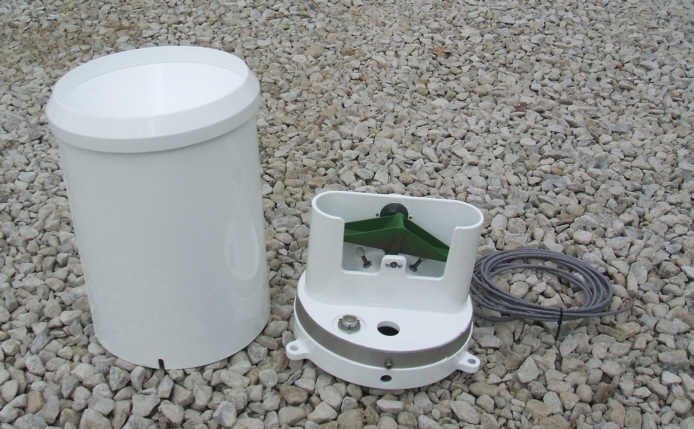
\includegraphics[width=.70\textwidth]{figures/TippingBucket.jpg}
  \caption{Tipping Bucket rain gauge.}
  \label{TippingBucket}
 \end{figure}


Figure:\ref{TippingBucket} shows the modern tipping rain gauge.
Modern tipping rain gauges consist of a plastic collector balanced over a pivot. When it tips, it actuates a switch (such as a reed switch) 
which is then electronically recorded or transmitted to a remote collection station.

\subsection{Optical rain gauge}
These have a row of collection funnels. In an enclosed space below each is a laser diode and a photo transistor detector. 
When enough water is collected to make a single drop, it drops from the bottom, falling into the laser beam path. 
The sensor is set at right angles to the laser so that enough light is scattered to be detected as a sudden flash of light. 
The flashes from these photo detectors are then read and transmitted or recorded.\cite{wiki}

 \begin{figure}[h]
 \centering
  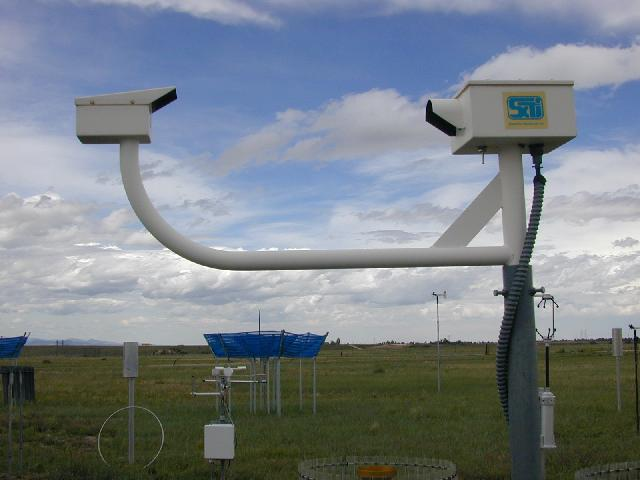
\includegraphics[height=6cm,width=.70\textwidth]{figures/optical_rain_gauge.jpg}
  \caption{Optical rain gauge.}
  \label{TOptical rain gauge}
 \end{figure}

\subsection{Measurement}
Most rain gauges generally measure the precipitation in millimetres equivalent to litres per square metre. The level of rainfall is sometimes reported as inches or centimetres.
\newline

Rain gauge amounts are read either manually or by automatic weather station (AWS). The frequency of readings will depend on the requirements of the collection agency.\cite{wiki} 


%---------------------------------------------------------------------------------------------------------------------\


\section{Water Level Sensor}
Wide spectrum of water level sensors is available in the market and commonly, they are classified on basis of:
\begin{itemize}
 \item Sensing points
 \item Measuring method
\end{itemize}

\subsection{Sensing Points}
\begin{enumerate}
 \item \textbf{Single Point Sensors:}\\
 These sensors are used where water level is to be sensed only at single location.
 \begin{figure}[h]
 \centering
  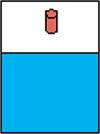
\includegraphics[width=.08\textwidth]{figures/wl_1.jpg}
  \caption{Single Point Sensors.}
  \label{Single Point Sensors}
 \end{figure} 
 
 \item \textbf{Multi-point Sensors:}\\
 These sensors are used where water level is to be sensed at number of locations single location.
 \begin{figure}[h]
 \centering
  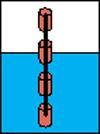
\includegraphics[width=.08\textwidth]{figures/wl_2.jpg}
  \caption{Multi-point Sensors.}
  \label{Multi-point Sensors}
 \end{figure} 
 
 \item \textbf{Continuous Sensors:}\\
 These sensors are used where water level at all locations is to sensed
 \begin{figure}[h]
 \centering
  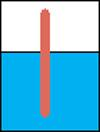
\includegraphics[width=.08\textwidth]{figures/wl_3.jpg}
  \caption{Continuous Sensors.}
  \label{Continuous Sensors}
 \end{figure} 
\end{enumerate}

\subsection{Measuring method}
\begin{enumerate}
 \item \textbf{Pressure Based Sensors}\\
 Pressure is defined as the force per unit area. The pressure at any depth, in a static fluid is equal to the weight of the liquid acting on a unit area 
 at that depth plus the pressure acting on the surface of the liquid.
 It relies on the principle that the difference between two pressures is equal to the height of the liquid multiplied by specific gravity.\cite{engi}
  \begin{figure}[h]
 \centering
  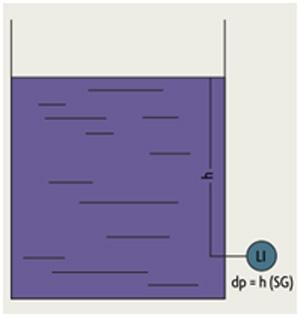
\includegraphics[width=.20\textwidth]{figures/wl_p.jpg}
  \caption{Pressure Based Sensors.}
  \label{Pressure Based Sensors}
 \end{figure} 
 \item \textbf{Ultrasonic Based Sensors}\\
 Ultrasonic level instruments operate on the basic time-of-flight principle using sound waves to determine liquid/solid/slurries level.
Ultrasonic Level sensors comprises of two elements; a high efficiency transducer and, an associated electronic transceiver. 
Complete return trip time between transmitted  ultrasonic pulse and reflected echo is measured to determine the water level.
 The frequency range for ultrasonic methods is in the range of 15 to 200 kHz.\cite{engi}
  \begin{figure}[h]
 \centering
  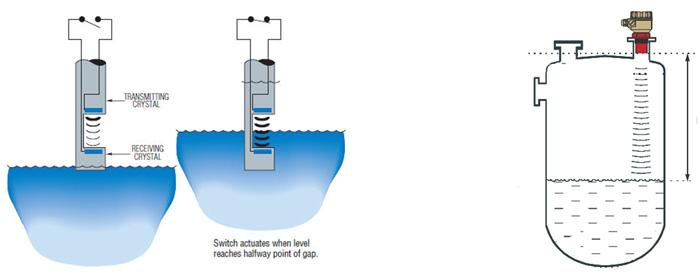
\includegraphics[width=.80\textwidth]{figures/wl_u.jpg}
  \caption{Ultrasonic Based Sensors.}
  \label{Ultrasonic Based Sensors}
 \end{figure} 
\end{enumerate}

\begin{table}[h]
\centering
\caption{Available Ultrasonic Level Sensor package comparison for experimental setup}
\begin{tabular}{||l|c|c|}\hline
\textbf{Attribute} &\textbf{HC-SR-04}	& \textbf{US-100} \\ \hline
Technology	& Ultrasonic & Ultrasonic\\ \hline
Min Range 	& 2 cm	& 2 cm \\ \hline
Max Range	& 4 m &	4 m	\\ \hline
Resolution	& 3 mm	& 1 mm \\ \hline
Measuring angle & Lees than 15 degree & lees than 15 degree \\ \hline
Frequency	& 40 KHz	& 40 KHz	\\ \hline
Availability	& More		& Less		\\ \hline
\end{tabular}
\end{table}

%---------------------------------------------------------------------------------------------------------------------



%---------------------------------------------------------------------------------------------------------------------
% References
%---------------------------------------------------------------------------------------------------------------------
\medskip

\nocite{*}
\bibliographystyle{ieeetr}
\bibliography{ref}
\addcontentsline{toc}{chapter}{\quad\,\,{\bibname}}
\label{chap:references}
%---------------------------------------------------------------------------------------------------------------------

%---------------------------------------------------------------------------------------------------------------------
%---------------------------------------------------------------------------------------------------------------------
\appendix
\chapter{LIST OF PUBLICATIONS}

% \newpagesquare root in late
% \includegraphics[angle=90,width=\textwidth, height=\textheight]{21061604_Certificate_Author_0.pdf}
% 
% \newpagesquare root in late
% \includegraphics[angle=-180,width=\textwidth]{figures/pgcon.jpg}

\end{document}          